\documentclass[11pt]{article}

% Codificación e idioma
\usepackage[utf8]{inputenc}
\usepackage[spanish,activeacute,es-tabla]{babel}

% Gráficos y flotantes
\usepackage{graphicx}
\usepackage{float}
\graphicspath{{imagenes/}}

% Márgenes y formato
\usepackage{anysize}
\marginsize{1.5cm}{1.5cm}{1cm}{1cm}

% Subfiguras y dibujo
\usepackage{subcaption}
\usepackage{tikz}

% Títulos y profundidad de numeración
\usepackage{titlesec}
\setcounter{secnumdepth}{4}
\titleformat{\paragraph}{\normalfont\normalsize\bfseries}{\theparagraph}{1em}{}
\titlespacing*{\paragraph}{0pt}{3.25ex plus 1ex minus .2ex}{1.5ex plus .2ex}

% Varios
\usepackage{svg}
\usepackage{titling}
\usepackage{enumitem}
\usepackage{wrapfig}
\usepackage{fancybox}

% Colores y matemáticas
\usepackage{xcolor}
\usepackage{amsmath}

% Tablas
\usepackage{array}
\usepackage{tabularx}
\usepackage{booktabs}
\usepackage{tocloft}

% Texto y enlaces
\usepackage{textcomp}
\usepackage[hidelinks]{hyperref}
\usepackage{hyphenat}

% Encabezados y pies
\usepackage{fancyhdr}
\setlength{\headheight}{14pt}

% Listados de código
\usepackage{listings}
\definecolor{codecomment}{rgb}{0.13,0.55,0.13}
\definecolor{codegray}{rgb}{0.5,0.5,0.5}
\definecolor{codepurple}{rgb}{0.58,0,0.82}
\definecolor{codebackground}{rgb}{0.97,0.97,0.97}
\definecolor{codeframe}{rgb}{0.7,0.7,0.7}
\lstdefinestyle{mystyle}{
  commentstyle=\color{codecomment},
  numberstyle=\tiny\color{codegray},
  stringstyle=\color{codepurple},
  basicstyle=\footnotesize\ttfamily,
  backgroundcolor=\color{codebackground},
  frame=single,
  rulecolor=\color{codeframe},
  breakatwhitespace=false,
  breaklines=true,
  captionpos=b,
  keepspaces=true,
  numbers=left,
  numbersep=5pt,
  showspaces=false,
  showstringspaces=false,
  showtabs=false,
  tabsize=3
}
\lstset{style=mystyle}
% Permitir caracteres acentuados (español) dentro de los entornos lstlisting
\lstset{
  literate=%
    {á}{{\'a}}1 {é}{{\'e}}1 {í}{{\'i}}1 {ó}{{\'o}}1 {ú}{{\'u}}1
    {Á}{{\'A}}1 {É}{{\'E}}1 {Í}{{\'I}}1 {Ó}{{\'O}}1 {Ú}{{\'U}}1
    {ñ}{{\~n}}1 {Ñ}{{\~N}}1 {ü}{{\"u}}1 {Ü}{{\"U}}1
    {¿}{{?`}}1 {¡}{{!`}}1
}
\usepackage[most]{tcolorbox}

%--------------------------------------------------------------------------------
% Comando auxiliar para reservar el espacio de las capturas.
% Reemplazar cada \placeholderfig{...} por el \includegraphics correspondiente
% una vez se suban las imágenes al proyecto de Overleaf.
%--------------------------------------------------------------------------------
\newcommand{\placeholderfig}[2][0.80\textwidth]{%
  \setlength{\fboxsep}{8pt}%
  \fbox{\parbox[c][4.2cm][c]{#1}{\centering\small\itshape #2}}}

%--------------------------------------------------------------------------------
% PORTADA
%--------------------------------------------------------------------------------
\begin{document}
\pagestyle{empty}

{\small
\noindent
\begin{tabular}{p{0.40\textwidth} p{0.50\textwidth}}

\includegraphics[scale=0.2]{usm.png} &

\includegraphics[scale=0.3]{elo.jpg}
\end{tabular}
}

\begin{center}
\rule{\linewidth}{0.5mm}\\[0.4cm]
{\Huge\textbf{Tarea: Emulando Redes con GNS3}}\\[0.25cm]
{\Large\textbf{Redes de Computadores II / Seminario de Redes de Computadores}}\\[0.5cm]
\rule{\linewidth}{0.5mm}\\[1.5cm]

{\Large
\begin{tabular}{rl}
\textbf{Fecha:}        & \today\\
\textbf{Integrantes:}  & Vicente Andrade; Ernesto Gamero; Matías Pérez\\
\textbf{Asignatura:}   & ELO323 / IPD438\\
\textbf{Profesor:}     & Agustín González V.\\
\textbf{Grupo:}        & 3\\
\end{tabular}
}
\end{center}

\clearpage

%--------------------------------------------------------------------------------
% ENCABEZADOS Y PIES
%--------------------------------------------------------------------------------
\pagestyle{fancy}
\fancyhf{}
\lhead{ELO323 / IPD438}
\rhead{\the\year}
\lfoot{USM 2026 - 2}
\rfoot{\thepage}
\renewcommand{\footrulewidth}{0.5pt}

%--------------------------------------------------------------------------------
% ÍNDICES
%--------------------------------------------------------------------------------
\begin{center}
\tableofcontents
\end{center}
\begin{center}
\listoffigures
\end{center}
\begin{center}
\listoftables
\end{center}

\clearpage

%================================================================================
\section{Desarrollo}
%================================================================================

Las topologías se armaron en GNS3 2.2.61 corriendo directamente sobre Linux, sin la GNS3 VM. Los terminales son VPCS, los switches son nodos Ethernet switch de GNS3, que conmutan en capa 2 sin cargar ningún sistema operativo, y el router es un Cisco 3725 emulado con dynamips.

\subsection{Familiarización con redes LAN}

\subsubsection{Crear LANs independientes (1.a)}

PC1 y PC2 quedaron conectados a Switch1, y PC3 y PC4 a Switch2. Entre los dos switches no hay enlace, de modo que cada uno es un dominio de broadcast aislado (Figura~\ref{fig:1a_topologia}). Las direcciones se asignaron a mano en la consola de cada VPCS, por ejemplo con \texttt{ip 192.168.0.102/24} en PC2, sin indicar gateway, y se revisaron con \texttt{show ip}.

\begin{figure}[H]
\centering
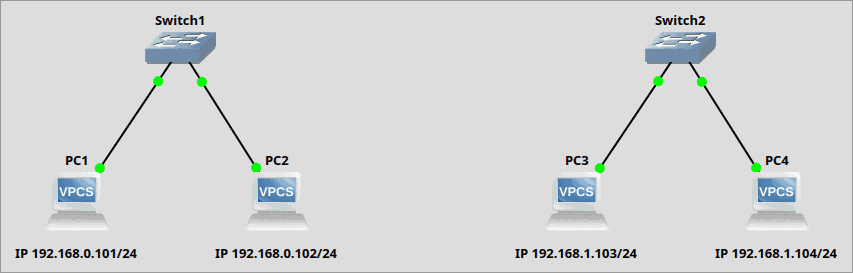
\includegraphics[width=0.70\textwidth]{1a_topologia.png}
\caption{Topología con dos LANs sin conexión entre sí (1.a).}
\label{fig:1a_topologia}
\end{figure}

\begin{wrapfigure}{r}{0.42\textwidth}
\vspace{-12pt}
\centering
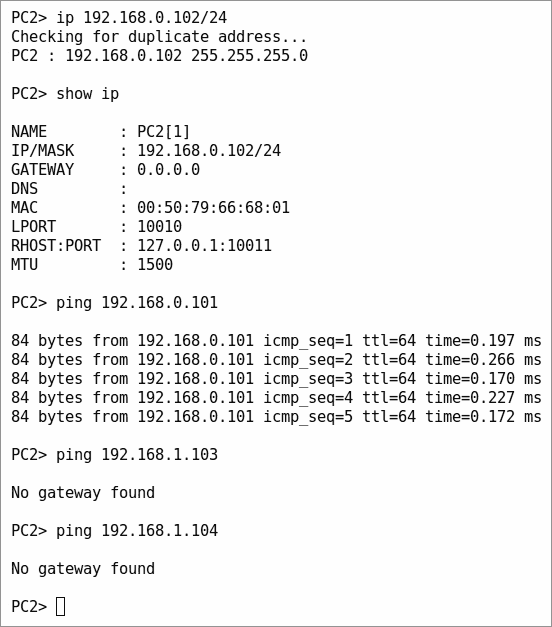
\includegraphics[width=0.40\textwidth]{1a_PC2_ip_ping.png}
\caption{Configuración de PC2 y pings hacia los otros VPCS (1.a).}
\label{fig:1a_ping}
\vspace{-10pt}
\end{wrapfigure}

El ping de PC2 a PC1 (192.168.0.101) recibió las cinco respuestas con TTL 64 y tiempos entre 0,17 y 0,27~ms (Figura~\ref{fig:1a_ping}). Hacia PC3 y PC4 el resultado fue \texttt{No gateway found}, y VPCS no llegó a enviar ningún paquete.

Antes de transmitir, PC2 aplica su máscara /24 al destino. Como 192.168.0.101 pertenece a su misma red, le basta resolver la MAC de PC1 por ARP y Switch1 entrega la trama directamente. En cambio 192.168.1.103 y 192.168.1.104 están fuera de 192.168.0.0/24, así que el paquete tendría que ir a un gateway, pero PC2 no tiene uno (\texttt{show ip} indica \texttt{GATEWAY: 0.0.0.0}). Aunque se hubiera configurado, nada en esta topología podría reenviar tráfico entre las dos redes, porque los switches no están unidos y ninguno trabaja en capa 3.

\subsubsection{Añadir un router (1.b)}

Con los VPCS apagados se agregó el router R1. Su template se importó desde el appliance \texttt{cisco-3725.gns3a} con la imagen \texttt{c3725-adventerprisek9-mz.124-15.T14} (IOS 12.4(15)T14), cuyo MD5 coincide con el que declara el appliance. Se conservó su valor de idle-PC (0x60c09aa0), sin el cual dynamips mantiene ocupado un núcleo completo del computador. La RAM se subió de 128 a 256~MB porque el material de ayuda lo pide para la pregunta 4. La interfaz FastEthernet0/0 (f0/0) se conectó al puerto e0 de Switch1 y la FastEthernet0/1 (f0/1) al e0 de Switch2.

En la consola (Figura~\ref{fig:1b_router}), cada interfaz recibió la primera dirección asignable de su red y un \texttt{no shutdown}, necesario porque en IOS las interfaces del router parten deshabilitadas (al arrancar aparecen como \textit{administratively down}). Después de ese comando, los mensajes \texttt{\%LINK-3-UPDOWN} y \texttt{\%LINEPROTO-5-UPDOWN} confirman que cada enlace quedó arriba.

Para el servicio DHCP se definió un pool por subred, LAN0 y LAN1. En cada uno, \texttt{network} fija la subred y la máscara que se entregan, y es lo que IOS usa para elegir el pool: la compara con la dirección de la interfaz por la que llega la solicitud. \texttt{default-router} define el gateway que recibirá el cliente y \texttt{dns-server} el servidor de nombres, que aquí es 8.8.8.8. El enunciado pide configurarlo aunque la red no tiene salida a Internet, así que ese valor no interviene en las pruebas. La dirección .1 de cada red, que ya ocupa el router, se excluyó del pool con \texttt{ip dhcp excluded-address}. La configuración se guardó en NVRAM con \texttt{copy running-config startup-config}, que respondió \texttt{[OK]}.

\begin{figure}[H]
\centering
\begin{subfigure}[t]{0.556\textwidth}
  \centering
  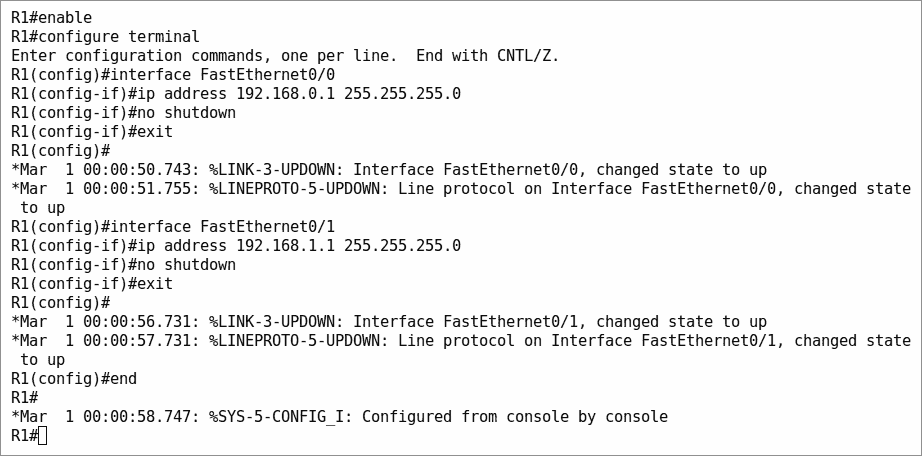
\includegraphics[width=\linewidth]{1b_R1_interfaces.png}
  \caption{Direcciones de las interfaces FastEthernet.}
\end{subfigure}\hfill
\begin{subfigure}[t]{0.41\textwidth}
  \centering
  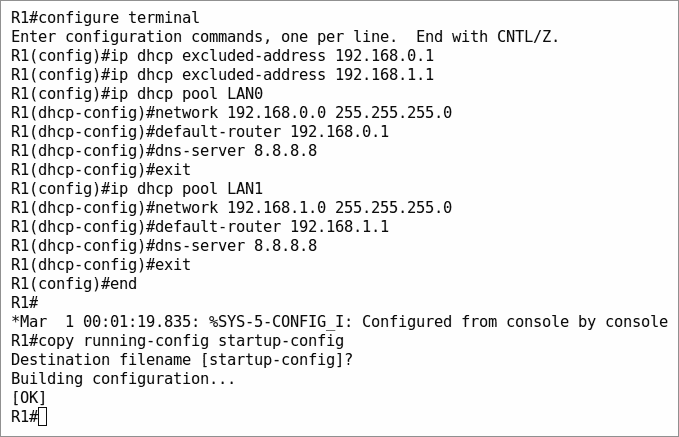
\includegraphics[width=\linewidth]{1b_R1_dhcp.png}
  \caption{Pools DHCP y respaldo de la configuración.}
\end{subfigure}
\caption{Comandos ejecutados en la consola de R1 (1.b).}
\label{fig:1b_router}
\end{figure}

\subsubsection{Asignación de direcciones IP por DHCP (1.c)}

Con R1 encendido, cada VPCS pidió su dirección con \texttt{ip dhcp}. La línea \texttt{DORA IP 192.168.0.2/24 GW 192.168.0.1} resume la negociación completa de PC1 (Figura~\ref{fig:1c_dhcp_a}), porque VPCS imprime una letra por cada mensaje del intercambio (Discover, Offer, Request y Ack). En \texttt{show ip} aparece también lo demás que entregó el servidor: DNS 8.8.8.8, la dirección del servidor DHCP y un arriendo de 86400~s, es decir, un día, que es el valor por defecto de IOS.

Las cuatro asignaciones se ven en la tabla de R1 (Figura~\ref{fig:1c_dhcp_b}). El Client-ID de cada entrada empieza con 01, el tipo de hardware Ethernet, y sigue con la MAC del VPCS (de 00:50:79:66:68:00 a 00:50:79:66:68:03), así que cada arriendo se puede asociar a su equipo. IOS fue asignando las direcciones de cada pool en orden ascendente; como se pidieron de PC1 a PC4, PC1 y PC3 quedaron con la .2 y PC2 y PC4 con la .3. Mientras R1 conserve esos arriendos, cada VPCS vuelve a recibir la misma dirección. Los arriendos viven solo en la RAM del router (no se configuró \texttt{ip dhcp database}), así que después de reiniciar R1 un orden distinto de solicitudes intercambiaría las direcciones. La Tabla~\ref{tab:direccionamiento} reúne las direcciones de esta etapa junto con las manuales de la pregunta 1.a.

\begin{table}[H]
\centering
\small
\caption{Direccionamiento de la red en la pregunta 1.}
\label{tab:direccionamiento}
\begin{tabular}{lllll}
\toprule
Equipo & Conexión & IP en 1.a (manual) & IP en 1.b y 1.c & Gateway en 1.c \\
\midrule
PC1    & Switch1 e1 & 192.168.0.101/24 & 192.168.0.2/24 (DHCP) & 192.168.0.1 \\
PC2    & Switch1 e2 & 192.168.0.102/24 & 192.168.0.3/24 (DHCP) & 192.168.0.1 \\
PC3    & Switch2 e1 & 192.168.1.103/24 & 192.168.1.2/24 (DHCP) & 192.168.1.1 \\
PC4    & Switch2 e2 & 192.168.1.104/24 & 192.168.1.3/24 (DHCP) & 192.168.1.1 \\
R1 f0/0 & Switch1 e0 & no existía      & 192.168.0.1/24 (manual) & no aplica \\
R1 f0/1 & Switch2 e0 & no existía      & 192.168.1.1/24 (manual) & no aplica \\
\bottomrule
\end{tabular}
\end{table}

Cada VPCS guardó su configuración con \texttt{save pc\_i.vpc}. El archivo contiene el nombre del equipo y la instrucción \texttt{dhcp}, sin la dirección, así que al cargarlo el VPCS vuelve a pedir una. La Figura~\ref{fig:1c_dhcp_c} lo muestra en PC1 después de apagarlo y encenderlo: \texttt{show ip} vuelve a 0.0.0.0/0 y, tras \texttt{load pc\_1.vpc}, el equipo recupera 192.168.0.2 porque R1 todavía tenía el arriendo asociado a su MAC. Los cuadros de texto del diagrama se actualizaron con la IP y el gateway de cada equipo (Figura~\ref{fig:1c_topologia}).

\begin{figure}[H]
\centering
\begin{minipage}[b]{0.52\textwidth}
  \centering
  \begin{subfigure}{\linewidth}
    \centering
    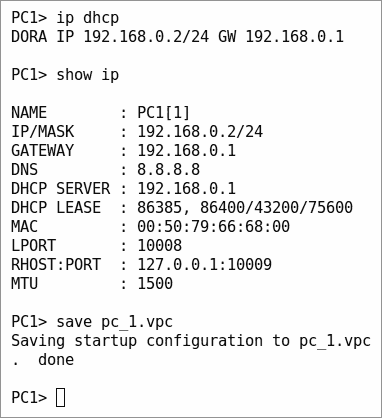
\includegraphics[width=0.534\linewidth]{1c_PC1_dhcp.png}
    \caption{\texttt{ip dhcp} y \texttt{save} en PC1.}\label{fig:1c_dhcp_a}
  \end{subfigure}\\[6pt]
  \begin{subfigure}{\linewidth}
    \centering
    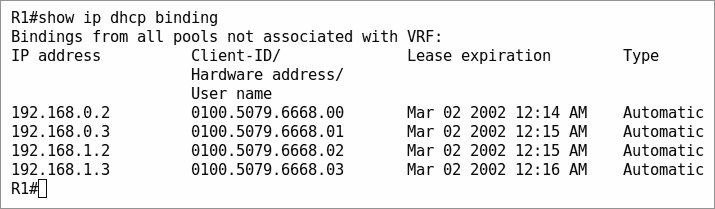
\includegraphics[width=\linewidth]{1c_R1_dhcp_binding.png}
    \caption{Arriendos registrados en R1.}\label{fig:1c_dhcp_b}
  \end{subfigure}
\end{minipage}\hspace{0.03\textwidth}%
\begin{minipage}[b]{0.265\textwidth}
  \centering
  \begin{subfigure}{\linewidth}
    \centering
    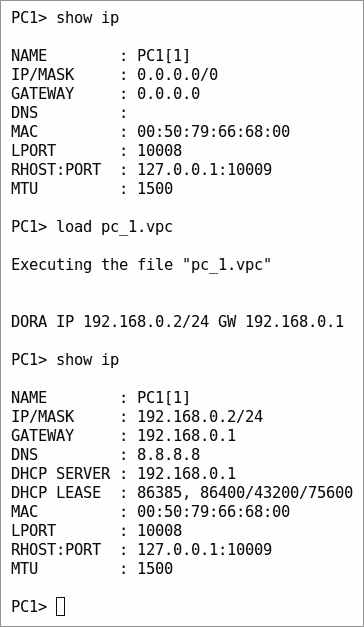
\includegraphics[width=\linewidth]{1c_PC1_load.png}
    \caption{\texttt{load} tras reiniciar PC1.}\label{fig:1c_dhcp_c}
  \end{subfigure}
\end{minipage}
\caption{Asignación de direcciones por DHCP (1.c).}
\label{fig:1c_dhcp}
\end{figure}

\begin{figure}[H]
\centering
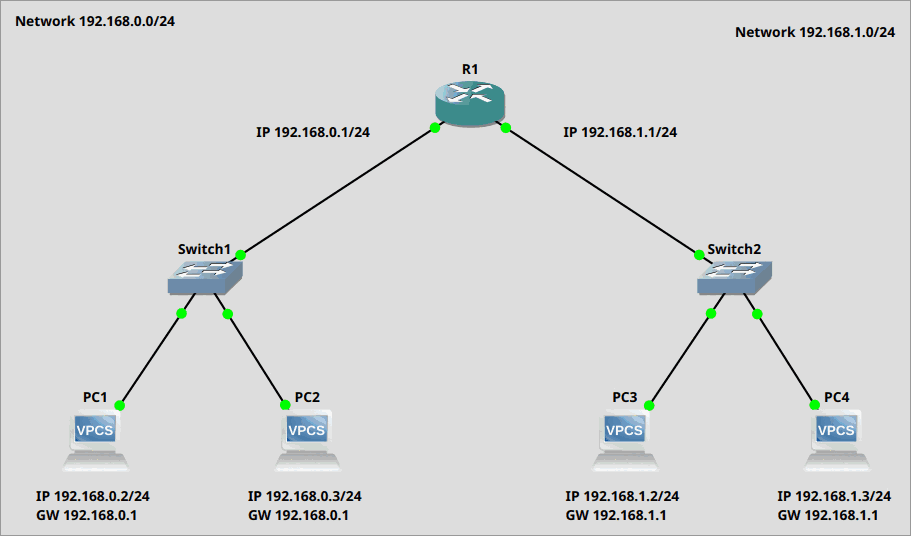
\includegraphics[width=0.72\textwidth]{1c_topologia.png}
\caption{Topología completa con las direcciones obtenidas por DHCP (1.c).}
\label{fig:1c_topologia}
\end{figure}

El proyecto se adjunta como \texttt{TAREA\_ELO323.IPD438\_parte1.gns3project}, exportado sin las imágenes base, que según el material de ayuda no es necesario incluir. Como GNS3 solo exporta con los nodos detenidos, antes se apagó R1; al detenerlo, GNS3 extrae la startup-config de su NVRAM y la escribe en \texttt{configs/i1\_startup-config.cfg}, de modo que lo que no se hubiera guardado con \texttt{copy running-config startup-config} no habría quedado en el proyecto. Del archivo se quitó la imagen \textit{ghost} de dynamips, una copia de 256~MB de la RAM del router con el IOS ya cargado, que GNS3 vuelve a generar al iniciar el router; sin ella el proyecto pesa 30~KB. La exportación se comprobó importándola como proyecto nuevo: R1 arrancó con sus interfaces y pools, y los cuatro VPCS traían su \texttt{pc\_i.vpc}. Para obtener las mismas direcciones de la Tabla~\ref{tab:direccionamiento} hay que encender R1, esperar a que IOS termine de cargar y ejecutar \texttt{load pc\_i.vpc} de PC1 a PC4.

\subsubsection{Pruebas de conectividad (1.d)}

Los tres pings desde PC2 recibieron todas sus respuestas (Figura~\ref{fig:1d_a}). VPCS muestra el TTL de la respuesta, que todos los VPCS emiten con 64. La de PC1 llega con ese valor y tarda menos de 0,5~ms porque el tráfico solo cruza Switch1. Las de PC3 y PC4 llegan con TTL 63, ya que R1, el único router del camino, lo descuenta en uno al reenviarlas de f0/1 a f0/0.

\begin{figure}[H]
\centering
\begin{subfigure}[t]{0.408\textwidth}
  \centering
  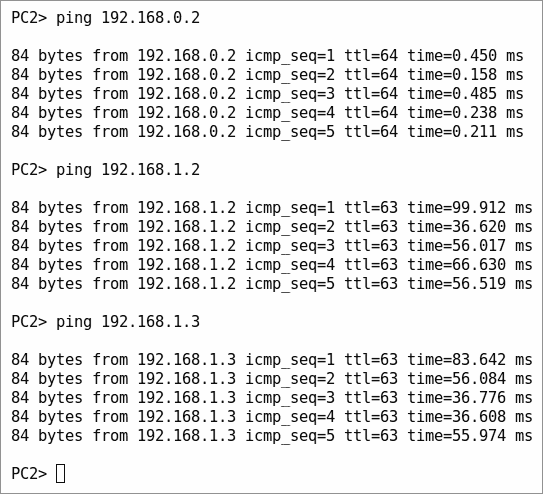
\includegraphics[width=\linewidth]{1d_PC2_ping.png}
  \caption{\texttt{ping} hacia PC1, PC3 y PC4.}\label{fig:1d_a}
\end{subfigure}\hfill
\begin{subfigure}[t]{0.562\textwidth}
  \centering
  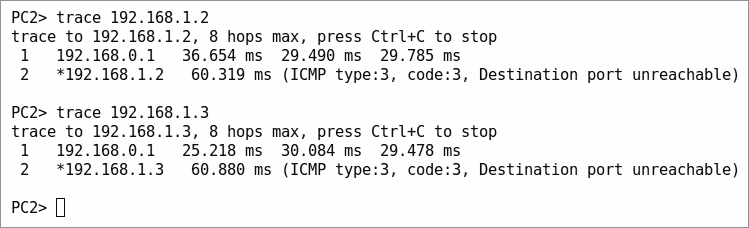
\includegraphics[width=\linewidth]{1d_PC2_trace.png}
  \caption{\texttt{trace} hacia PC3 y PC4.}\label{fig:1d_b}
\end{subfigure}
\caption{Pruebas de conectividad desde PC2 (1.d).}
\label{fig:1d}
\end{figure}

El \texttt{trace} de la Figura~\ref{fig:1d_b} confirma la ruta, con 192.168.0.1 como primer salto y el destino como segundo. VPCS antepone un asterisco a las respuestas que son mensajes ICMP de error, y el paréntesis indica cuál: tipo 3, código 3, puerto inalcanzable. Como VPCS sondea con UDP hacia un puerto cerrado, ese mensaje lo envía el propio PC3 o PC4 y prueba que la sonda llegó. Una sonda sin respuesta aparecería como un asterisco aislado, y aquí no hubo ninguna.

Los tiempos entre LANs, de 36,6 a 99,9~ms, los agrega el router emulado. El \texttt{trace} lo confirma, porque R1 tarda entre 25 y 37~ms en responder como primer salto, sin que el paquete llegue a la otra LAN. Dynamips emula por software la CPU MIPS del 3725 y, con el idle-PC configurado, la suspende cuando IOS está ocioso; ambas cosas retrasan el reenvío, aunque no se hicieron pruebas para separar cuánto aporta cada una.

En ninguno de los pings se perdió el primer paquete. Si R1 hubiera tenido que resolver por ARP la MAC del destino en ese momento, IOS habría descartado el paquete que disparó la consulta y VPCS habría mostrado \texttt{icmp\_seq=1 timeout}. Lo más probable es que R1 ya conociera las MAC de PC3 y PC4 por el tráfico anterior, aunque su tabla ARP no se revisó antes de las pruebas.


\subsection{Simulación de enlaces ideales y reales}

La red de la Figura 3 del enunciado se armó en un proyecto GNS3 separado del de la pregunta 1. Los tres terminales son máquinas Alpine, creadas con el template que indica el material de ayuda (512~MB de RAM y \texttt{-cpu qemu64}), y el enlace con limitaciones es una VM NETem 0.4.1 intercalada entre Switch2 y PC3. PC1 está conectado a Switch1, PC2 a Switch2, y ambos switches están unidos entre sí. Las direcciones, de 192.168.0.1 a 192.168.0.3, se asignaron a mano con \texttt{ip addr add 192.168.0.x/24 dev eth0} e \texttt{ip link set eth0 up}. Además, a cada máquina se le cambió el nombre con \texttt{hostname} para distinguir las consolas en las capturas. En GNS3 los nodos conservan el nombre que les dio el template, de Alpine-ELO323-1 a Alpine-ELO323-3, y los cuadros de texto de la Figura~\ref{fig:2_topologia} indican a qué PC corresponde cada uno y qué dirección tiene.

\begin{figure}[H]
\centering
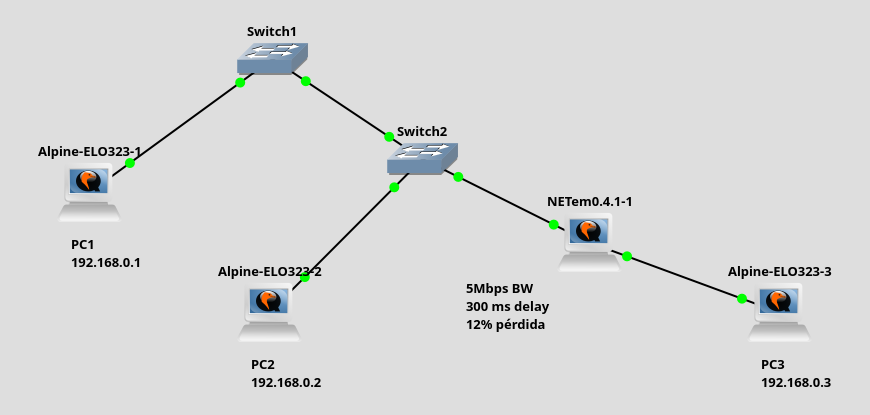
\includegraphics[width=0.72\textwidth]{2_topologia.png}
\caption{Topología de la pregunta 2 en GNS3, con las direcciones y la configuración del enlace NETem.}
\label{fig:2_topologia}
\end{figure}

En el menú de NETem se configuró el sentido eth0 a eth1 con los valores de la Tabla 1 del enunciado (5000~kbit/s, 300~ms de retardo y 12\,\% de pérdida, sin jitter), y el sentido contrario quedó en la opción \textit{Symmetric}, que copia la misma configuración. El Código~\ref{lst:tc} muestra cómo quedó aplicada en la VM. Cada interfaz tiene un limitador TBF a 5000~kbit/s y, debajo, un qdisc netem que agrega el retardo y la pérdida. La pérdida aparece como modelo de Gilbert-Elliott con $p = 12$\,\% y $r = 88$\,\%; como $p + r = 1$, la probabilidad de pasar al estado de pérdida es 12\,\% tanto desde el estado bueno como desde el malo, así que cada paquete se pierde con esa probabilidad sin importar lo que le pasó al anterior.

\renewcommand{\lstlistingname}{Código}
\begin{lstlisting}[numbers=none, basicstyle=\scriptsize\ttfamily, caption={Configuración aplicada por NETem en sus dos interfaces.}, label=lst:tc]
gns3@box:~$ tc qdisc show
qdisc tbf 1: dev eth0 root refcnt 2 rate 5000Kbit burst 1600b lat 20.0ms
qdisc netem 10: dev eth0 parent 1:1 limit 1000 delay 300.0msloss gemodel p 12% r 88% 1-h 0% 1-k 0%
qdisc tbf 1: dev eth1 root refcnt 2 rate 5000Kbit burst 1600b lat 20.0ms
qdisc netem 10: dev eth1 parent 1:1 limit 1000 delay 300.0msloss gemodel p 12% r 88% 1-h 0% 1-k 0%
\end{lstlisting}

\subsubsection{Pruebas de conectividad (2.a)}

Desde PC2, los diez pings a PC1 volvieron todos, con TTL 64 y tiempos entre 1,2 y 1,9~ms (Figura~\ref{fig:2_a}). Hacia PC3 volvieron nueve de diez, y salvo el primero tardaron entre 602,3 y 603,3~ms. El retardo configurado se cumple: cada ping cruza NETem a la ida y a la vuelta, lo que suma $2 \times 300 = 600$~ms. Los 2 a 3~ms restantes corresponden al paso por los switches y las máquinas virtuales, que hacia PC1 ya toma entre 1,2 y 1,9~ms, más la transmisión de cada trama a 5~Mbit/s.

El primer ping a PC3 tardó 1205~ms porque PC2 todavía no conocía la MAC de PC3 y tuvo que pedirla por ARP. La consulta y su respuesta también cruzan NETem, así que el echo salió recién unos 600~ms después. El paquete perdido de los diez no sirve como estimación de la pérdida del enlace, porque con tan pocas muestras el resultado varía mucho de una prueba a otra; esa estimación se hace en la pregunta 2.b.

\begin{figure}[H]
\centering
\begin{subfigure}[t]{0.445\textwidth}
  \centering
  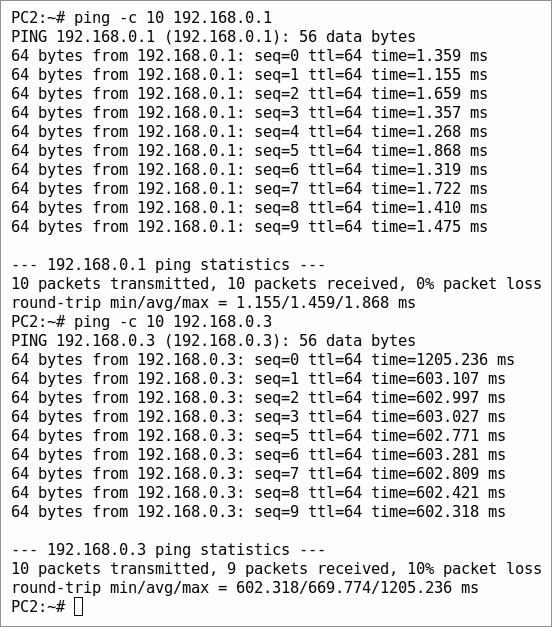
\includegraphics[width=\linewidth]{2a_PC2_ping.png}
  \caption{Pings de PC2 a PC1 y PC3 (2.a).}\label{fig:2_a}
\end{subfigure}\hfill
\begin{subfigure}[t]{0.535\textwidth}
  \centering
  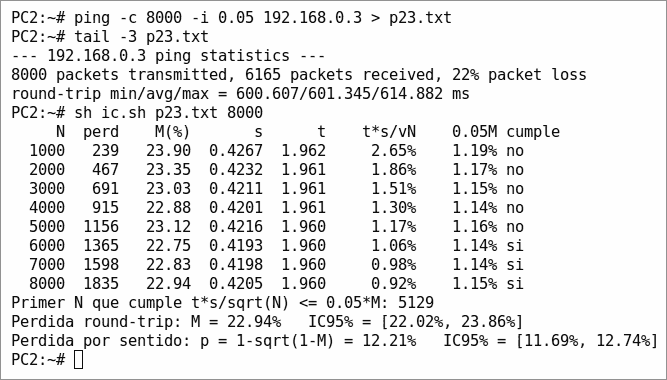
\includegraphics[width=\linewidth]{2b_PC2_perdidas.png}
  \caption{Medición de pérdidas hacia PC3 y cálculo del intervalo (2.b).}\label{fig:2_b}
\end{subfigure}
\caption{Pruebas desde PC2 en la red con el enlace NETem.}
\label{fig:2}
\end{figure}

\subsubsection{Intervalos de confianza (2.b)}

La estimación sigue el apunte del curso sobre pérdidas round-trip. Cada ping es un experimento binario, con $x_i = 1$ si el paquete se pierde, de modo que con $k$ pérdidas en $N$ envíos
\begin{equation}
M = \frac{k}{N}, \qquad s^2 = \frac{k}{N-1}\left(1 - \frac{k}{N}\right),
\end{equation}
y el intervalo de confianza es $M \pm t\,s/\sqrt{N}$, con $t$ de la distribución t de Student para $N-1$ grados de libertad y 95\,\% de confianza. El apunte define el intervalo de $\pm 5$\,\% en forma relativa a la media, así que hay que reunir mediciones hasta que
\begin{equation}
t\,\frac{s}{\sqrt{N}} \le 0{,}05\,M .
\label{eq:criterio}
\end{equation}

Si NETem pierde 12\,\% en cada sentido, el ping debería perder $1 - (1 - 0{,}12)^2 = 22{,}56$\,\% de los paquetes. Con ese valor y $t \approx 1{,}96$, la condición (\ref{eq:criterio}) se cumple desde unos 5300 envíos, de modo que se mandaron 8000 con \texttt{ping -c 8000 -i 0.05}. A 20 paquetes por segundo la prueba tomó unos siete minutos y generó unos 16~kbit/s, muy por debajo de los 5~Mbit/s del enlace, por lo que el limitador no descartó paquetes por su cuenta. La salida quedó en un archivo que procesa el script del Código~\ref{lst:ic}: marca como perdido cada número de secuencia sin respuesta y cada 1000 envíos calcula $M$, $s$, $t$ y el semiancho del intervalo. El valor de $t$ sale de una expansión de la t de Student en función de los grados de libertad.

\begin{lstlisting}[basicstyle=\scriptsize\ttfamily, caption={Script \texttt{ic.sh} que calcula el intervalo de confianza en PC2.}, label=lst:ic]
#!/bin/sh
# ic.sh <salida_de_ping> <N>: IC 95% de la perdida round-trip segun el apunte (experimento binario)
grep -o 'seq=[0-9]*' "$1" | cut -d= -f2 | awk -v N="$2" '
function tq(df,  z) { z = 1.959964; return z + (z*z*z + z)/(4*df) + (5*z*z*z*z*z + 16*z*z*z + 3*z)/(96*df*df) }
{ ok[$1] = 1 }
END {
  printf "%6s %5s %7s %7s %6s %9s %8s %s\n", "N", "perd", "M(%)", "s", "t", "t*s/vN", "0.05M", "cumple"
  k = 0; first = 0
  for (i = 0; i < N; i++) {
    if (!(i in ok)) k++
    n = i + 1
    if (n < 30) continue
    M = k/n; s = sqrt(k/(n-1)*(1 - k/n)); t = tq(n-1); h = t*s/sqrt(n)
    if (h <= 0.05*M && !first) first = n
    if (n % 1000 == 0) printf "%6d %5d %7.2f %7.4f %6.3f %8.2f%% %7.2f%% %s\n", n, k, 100*M, s, t, 100*h, 5*M, (h <= 0.05*M ? "si" : "no")
  }
  printf "Primer N que cumple t*s/sqrt(N) <= 0.05*M: %d\n", first
  printf "Perdida round-trip: M = %.2f%%   IC95%% = [%.2f%%, %.2f%%]\n", 100*M, 100*(M-h), 100*(M+h)
  printf "Perdida por sentido: p = 1-sqrt(1-M) = %.2f%%   IC95%% = [%.2f%%, %.2f%%]\n", 100*(1-sqrt(1-M)), 100*(1-sqrt(1-(M-h))), 100*(1-sqrt(1-(M+h)))
}'
\end{lstlisting}

Se perdieron 1835 de los 8000 paquetes (Figura~\ref{fig:2_b}), lo que da $M = 22{,}94$\,\% con $s = 0{,}4205$ y $t = 1{,}960$. El semiancho del intervalo es de 0,92 puntos porcentuales, menor que $0{,}05\,M = 1{,}15$, y la condición se cumplió por primera vez con $N = 5129$; en la tabla, a los 5000 envíos todavía no se cumplía (1,17 frente a 1,16). Con 95\,\% de confianza, la pérdida de ida y vuelta está entre 22,02\,\% y 23,86\,\%.

El 22\,\% que informa ping es mayor que el 12\,\% configurado porque ping mide ida y vuelta y NETem aplica la pérdida en cada sentido. Un paquete que se pierde a la ida ya no puede perderse a la vuelta, de modo que la pérdida round-trip vale $P_{rt} = 2p - p^2$, algo menos que $2p$. Despejando, como indica el apunte,
\begin{equation}
p = 1 - \sqrt{1 - P_{rt}} ,
\end{equation}
se obtiene una pérdida por sentido de 12,21\,\%, con intervalo de 11,69\,\% a 12,74\,\% al aplicar la misma fórmula a los extremos. El 12\,\% configurado queda dentro, de modo que la pérdida medida en cada sentido es igual a la configurada con la precisión pedida. Lo mismo pasa con el valor esperado de ida y vuelta, 22,56\,\%, que cae dentro de su intervalo.

El intervalo supone que los envíos son independientes, y los datos lo confirman. La fracción de pérdidas fue 0,230 cuando el paquete anterior se había perdido y 0,229 cuando había llegado, y las rachas de 1, 2 y 3 pérdidas seguidas (1087, 252 y 59) coinciden con las que daría un proceso independiente con la misma tasa (1090, 250 y 57). Las 6165 respuestas tuvieron un RTT entre 600,6 y 614,9~ms, con promedio de 601,3~ms, lo que confirma también el retardo de 300~ms por sentido.

\subsubsection{Mediciones de throughput (2.c)}

En PC1 se dejó corriendo el servidor de iperf 2.2.0 con \texttt{iperf -s}, y desde PC2 y PC3 se ejecutó \texttt{iperf -c 192.168.0.1}, con \texttt{-t} para fijar la duración de la prueba e \texttt{-i} para que el cliente informe la tasa de cada intervalo. Por defecto iperf usa TCP: el cliente abre una conexión, escribe datos en ella tan rápido como TCP los acepta y, al terminar, cada extremo informa cuántos bytes pasaron y a qué tasa\footnote{Como en iperf, 1~KB son 1024~bytes y 1~kbit/s son 1000~bit/s.}.

PC2 alcanzó 1,26~Gbit/s durante 30~s, con intervalos de 5~s entre 1,21 y 1,30~Gbit/s (Figura~\ref{fig:2c_tcp_a}). Su camino hacia PC1 solo cruza los dos switches, donde no hay ningún límite configurado. Cada trama viaja entre los procesos QEMU de las máquinas y los procesos dynamips que emulan los switches como un datagrama UDP del propio computador, así que esa tasa depende del procesamiento disponible y no de un enlace.

Desde PC3 se hicieron tres pruebas de 60~s (Tabla~\ref{tab:2c_tcp}). Según el servidor, PC3 transfirió entre 465 y 686~KB, a 56,8, 62,6 y 74,1~kbit/s, con un promedio de 64,5~kbit/s. La tasa medida resultó mucho menor que los 5~Mbit/s configurados en NETem, apenas entre 1,1 y 1,5\,\% de ellos.

\begin{table}[H]
\centering
\small
\caption{Pruebas TCP de 60~s desde PC3 hacia PC1 (2.c).}
\label{tab:2c_tcp}
\begin{tabular}{lccccc}
\toprule
 & \multicolumn{2}{c}{Cliente (PC3)} & \multicolumn{3}{c}{Servidor (PC1)} \\
\cmidrule(lr){2-3}\cmidrule(lr){4-6}
Prueba & Duración (s) & Tasa (kbit/s) & Duración (s) & Recibido (KB) & Tasa (kbit/s) \\
\midrule
1 & 77,91 & 72,1 & 75,85 & 686 & 74,1 \\
2 & 67,72 & 56,3 & 67,10 & 465 & 56,8 \\
3 & 73,68 & 62,1 & 73,06 & 559 & 62,6 \\
\midrule
Promedio & & & & & 64,5 \\
\bottomrule
\end{tabular}
\end{table}

En las tres pruebas el cliente siguió activo más de 60~s, hasta 77,9~s en la primera, y en la segunda y la tercera sus intervalos muestran bloques de 63,6~KB o cero bytes. Pasa porque el cliente cuenta los bytes que entrega a su socket TCP, no los que llegan a PC1. Mientras el búfer de envío tiene espacio la escritura es inmediata, y por eso en los primeros 10~s de la primera prueba el cliente alcanzó a escribir 368~KB (Figura~\ref{fig:2c_tcp_b}), aunque en ese lapso solo llegaron 225~KB a PC1. Cuando el búfer se llena, el cliente queda bloqueado hasta que TCP libera espacio. Al cumplirse los 60~s el búfer todavía guardaba datos y la conexión se cerró recién cuando terminaron de llegar. La tasa válida es entonces la que calcula el servidor (Figura~\ref{fig:2c_tcp_c}), que cuenta lo que efectivamente recibió.

\begin{figure}[H]
\centering
\begin{subfigure}[t]{0.49\textwidth}
  \centering
  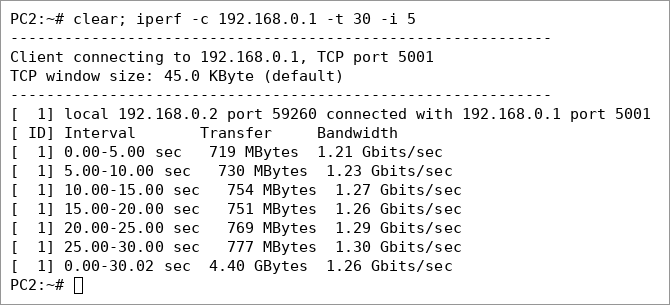
\includegraphics[width=\linewidth]{2c_PC2_iperf_tcp.png}
  \caption{Cliente en PC2.}\label{fig:2c_tcp_a}
\end{subfigure}\hfill
\begin{subfigure}[t]{0.49\textwidth}
  \centering
  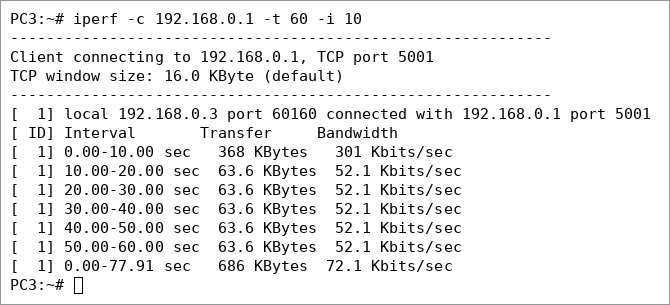
\includegraphics[width=\linewidth]{2c_PC3_iperf_tcp.png}
  \caption{Cliente en PC3, primera prueba.}\label{fig:2c_tcp_b}
\end{subfigure}\\[6pt]
\begin{subfigure}[t]{0.49\textwidth}
  \centering
  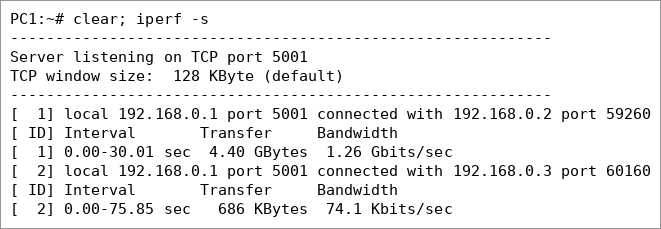
\includegraphics[width=\linewidth]{2c_PC1_iperf_server_tcp.png}
  \caption{Servidor en PC1.}\label{fig:2c_tcp_c}
\end{subfigure}
\caption{Mediciones de throughput con TCP (2.c).}
\label{fig:2c_tcp}
\end{figure}

El límite de 5~Mbit/s no es lo que frena a TCP. Una conexión TCP envía como máximo una ventana de datos por cada RTT, así que su tasa es aproximadamente la ventana dividida por el RTT. Con 600~ms de RTT, llenar 5~Mbit/s exigiría tener $5 \cdot 10^6 \times 0{,}6 / 8 = 375\,000$~bytes en vuelo, unos 259 segmentos de 1448~bytes. Para ver qué ventana usó TCP en la práctica, durante la primera prueba se capturó el tráfico del enlace entre NETem y PC3 desde GNS3, y la captura se analizó con tshark.

PC3 envió 539 segmentos de datos, 486 distintos y 53 retransmisiones (9,8\,\% de los envíos, cerca del 12\,\% de pérdida configurado). TCP interpreta cada pérdida como una señal de congestión. Treinta y seis de ellas se recuperaron con retransmisión rápida, después de recibir ACK duplicados con bloques SACK, y en ese caso CUBIC, el control de congestión que usa Linux por defecto, reduce la ventana al 70\,\%. Las otras 17 se detectaron al vencer el temporizador de retransmisión (RTO), entre 0,6 y 2,5~s después del envío original, y entonces la ventana vuelve a un segmento. Como se pierde aproximadamente uno de cada ocho segmentos, la ventana no alcanza a crecer entre una reducción y la siguiente. En los primeros 10~s, mientras TCP crecía en \textit{slow start} desde su ventana inicial de 10 segmentos, hubo en promedio 12,6 segmentos en vuelo (enviados y sin confirmar), con un máximo de 26. Desde ahí hasta el final el promedio bajó a 1,4 segmentos y nunca pasó de 10. La ventana que anunciaba PC1 estuvo siempre entre 43 y 318~KB, por encima de lo que había en vuelo, de modo que el receptor no fue el límite.

Los ACK de PC1 muestran el mismo cambio. Confirmaron 225~KB en los primeros 10~s, es decir 184~kbit/s, y entre 48 y 82~KB en cada intervalo de 10~s posterior, entre 39 y 67~kbit/s. Por eso la primera prueba promedió 74,1~kbit/s: el resultado de iperf incluye ese arranque, y en régimen permanente TCP se mantuvo cerca de 54~kbit/s. El modelo de Mathis et al.\footnote{M. Mathis, J. Semke, J. Mahdavi y T. Ott, ``The macroscopic behavior of the TCP congestion avoidance algorithm'', \textit{ACM SIGCOMM Computer Communication Review}, vol.~27, n.º~3, pp.~67--82, 1997.} estima la tasa de TCP en régimen con pérdidas aleatorias como
\begin{equation}
B \approx \frac{\mathrm{MSS}}{\mathrm{RTT}} \cdot \frac{C}{\sqrt{p}} ,
\end{equation}
con $C = \sqrt{3/2}$ si el receptor confirma cada segmento y $C = \sqrt{3/4}$ si confirma uno de cada dos. Con MSS de 1448~bytes, RTT de 0,6~s y $p = 0{,}12$ se obtienen entre 48 y 68~kbit/s, y los 54~kbit/s medidos caen en ese rango. El modelo no considera los RTO, pero muestra lo esencial: en la expresión no aparece el ancho de banda del enlace, porque la tasa de TCP la determinan la pérdida y el RTT.

Para comprobar que el enlace sí entrega los 5~Mbit/s, la medición desde PC3 se repitió con UDP, que no tiene control de congestión y transmite a la tasa pedida sin esperar confirmaciones. En PC1 se levantó \texttt{iperf -s -u}, y PC3 envió datagramas de 1470~bytes durante 30~s, primero a 5~Mbit/s (\texttt{-u -b 5m}) y luego a 10~Mbit/s (Figura~\ref{fig:2c_udp}). El informe que el servidor devuelve al cliente llegó con la pérdida en 0\,\% en la primera prueba y no llegó en la segunda, así que los resultados se tomaron directamente del servidor.

\begin{figure}[H]
\centering
\begin{subfigure}[t]{0.49\textwidth}
  \centering
  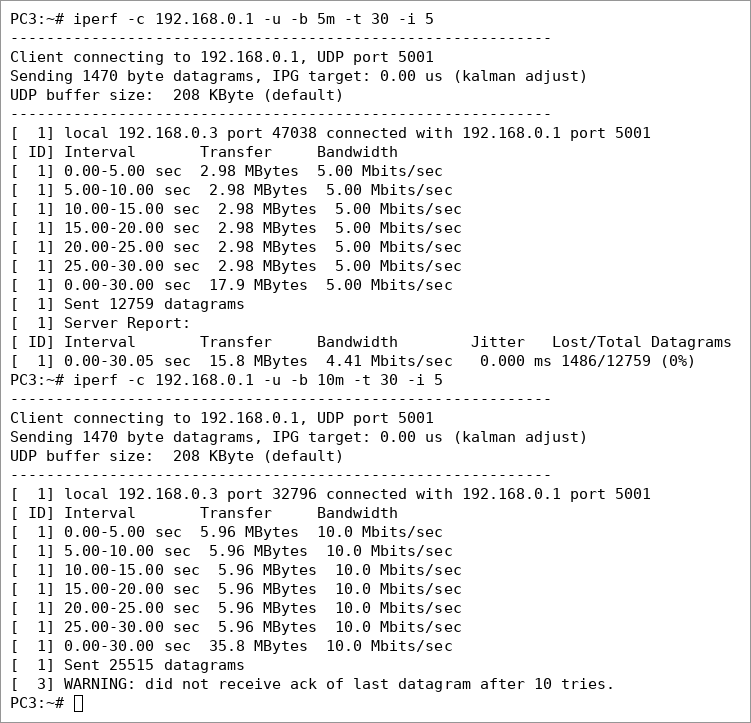
\includegraphics[width=\linewidth]{2c_PC3_iperf_udp.png}
  \caption{Cliente en PC3.}\label{fig:2c_udp_a}
\end{subfigure}\hfill
\begin{subfigure}[t]{0.49\textwidth}
  \centering
  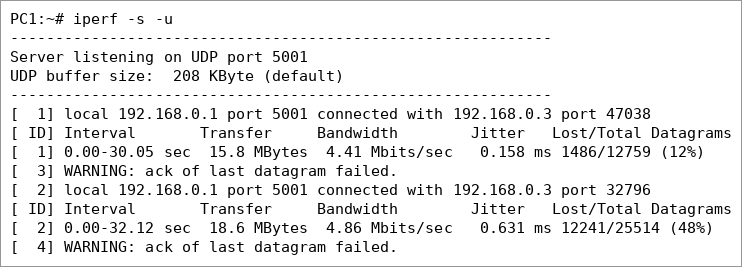
\includegraphics[width=\linewidth]{2c_PC1_iperf_server_udp.png}
  \caption{Servidor en PC1.}\label{fig:2c_udp_b}
\end{subfigure}
\caption{Mediciones de throughput con UDP desde PC3 (2.c).}
\label{fig:2c_udp}
\end{figure}

A 5~Mbit/s llegaron 4,41~Mbit/s y se perdieron 1486 de 12759 datagramas, un 11,6\,\%, que coincide con el 12\,\% configurado (Figura~\ref{fig:2c_udp_b}). No hubo otros descartes: NETem elimina cada datagrama con probabilidad 12\,\% antes de entregarlo al limitador, y lo que queda, unos 4,5~Mbit/s contando las cabeceras, no alcanza a llenar los 5000~kbit/s. A 10~Mbit/s llegaron 4,86~Mbit/s y se perdió el 48\,\% de los datagramas. El limitador TBF cuenta la trama completa, de 1512~bytes (1470 de datos, 8 de UDP, 20 de IP y 14 de Ethernet), y 5000~kbit/s de tramas equivalen a $5000 \times 1470 / 1512 = 4861$~kbit/s de datos, justo lo medido. Lo que excede esa tasa se acumula en la cola de NETem, de 1000 paquetes, y se descarta cuando la cola está llena. Esa misma cola explica que el servidor siguiera recibiendo unos 2~s después de que el cliente dejó de enviar.

Desde PC3, entonces, TCP obtuvo mucho menos que lo configurado, entre 57 y 74~kbit/s frente a 5~Mbit/s, aunque el enlace es capaz de entregarlo, como muestra el tope de 4,86~Mbit/s alcanzado con UDP. El valor de Bandwidth de NETem es un máximo, y TCP queda lejos de él porque, con 12\,\% de pérdida y 600~ms de RTT, su control de congestión mantiene la ventana en unos pocos segmentos. UDP, que no se frena, tampoco supera la tasa configurada: entrega 4,41~Mbit/s útiles al ofrecer 5~Mbit/s, por la pérdida, y nunca más de 4,86~Mbit/s, por las cabeceras.

\end{document}
